% Vorlage: https://www.pfsr.de/latex

% -- Anfang Präambel
\documentclass[german,  % Standardmäßig deutsche Eigenarten, englisch -> english
parskip=full,  % Absätze durch Leerzeile trennen
%bibliography=totoc,  % Literatur im Inhaltsverzeichnis (ist unüblich)
%draft,  % TODO: Entwurfsmodus -> entfernen für endgültige Version
]{scrartcl}

\usepackage[utf8]{inputenc}  % Kodierung der Datei
\usepackage[T1]{fontenc}  % Vollen Umfang der Schriftzeichen
\usepackage[ngerman]{babel}  % Sprache auf Deutsch (neue Rechtschreibung)

% Mathematik und Größen
\usepackage{amsmath}
\usepackage[locale=DE,  % deutsche Eigenarten, englisch -> US
separate-uncertainty,  % Unsicherheiten seperat angeben (mit ±)
]{siunitx}
\usepackage{physics}  % Erstellung von Gleichungen vereinfachen

\usepackage{graphicx}  % Bilder einbinden \includegraphics{Pfad/zur/Datei(ohne Dateiendung)}

% Gestaltung
\usepackage{booktabs}  % schönere Tabellen
\usepackage[toc]{multitoc}  % mehrspaltiges Inhaltsverzeichnis
\usepackage{csquotes}  % Anführungszeichen mit \enquote
\usepackage{caption}  % Anpassung der Bildunterschriften, Tabellenüberschriften
\usepackage{subcaption}  % Unterabbildungen, Untertabellen, …
\usepackage{enumitem}  % Listen anpassen
\setlist{itemsep=-10pt}  % Abstände zwischen Listenpunkten verringern

% Manipulation des Seitenstils
\usepackage[headtopline = .5pt]{scrlayer-scrpage}

% Bibliographie
\usepackage[backend=biber]{biblatex}
\addbibresource{bibliography.bib}

% SI-Einheiten darstellen
\usepackage{siunitx}

% Kopf-/Fußzeilen setzen
\pagestyle{scrheadings}  % Stil für die Seite setzen
\clearmainofpairofpagestyles  % Stil zurücksetzen, um ihn neu zu definieren
\automark{section}  % Abschnittsnamen als Seitenbeschriftung verwenden
\ofoot{\pagemark}  % Seitenzahl außen in Fußzeile
\ihead{\headmark}  % Seitenbeschriftung mittig in Kopfzeile

\usepackage[hidelinks]{hyperref}  % Links und weitere PDF-Features

% TODO: Titel und Autor, … festlegen
\newcommand*{\titel}{Auswertung von pp-Kollisionsereignissen}
\newcommand*{\autor}{Sebastian Thiede, Alexander Lettau}
\newcommand*{\abk}{PP}
\newcommand*{\betreuer}{Max Märker}
\newcommand*{\messung}{02.12.2021 \& 09.11.2021}
\newcommand*{\ort}{ASB/429}

\hypersetup{pdfauthor={\autor}, pdftitle={\titel}}  % PDF-Metadaten setzen

% automatischen Titel konfigurieren
\titlehead{Praktikum des IKTP \abk \hfill TU Dresden}
\subject{Versuchsprotokoll}
\title{\titel}
\author{\autor}
\date{\begin{tabular}{ll}
Protokoll: & \today\\
Messung: & \messung\\
Ort: & \ort\\
Betreuer: & \betreuer\end{tabular}}

% -- Ende Präambel

\begin{document}
\begin{titlepage}
\maketitle  % Titel setzen
\tableofcontents  % Inhaltsverzeichnis setzen
\end{titlepage}

% ----- DOKUMENT ANFANG -----

\section{Aufgabenstellung}
Die Beschleunigermas­senspektrometrie (AMS) ist ein wichtiges Werkzeug zur Trennung und Detektierung von Nukliden.
Eine der häufigsten Anwendungen ist die Altersbestimmung von Proben aus der Natur durch Messung der Konzentration verschiedener Nuklide, die auf der Erdoberfläche durch kosmische Strahlung entstehen.
Im Gegensatz zu anderen Verfahren der Massenspektrometrie erreicht man bei der AMS eine sehr gute Unterdrückung atomarer und molekularer Isobare.
Die Messzeiten sind relativ kurz und es lassen sich auch kleine Proben untersuchen.

In diesem Versuch wurde der Beschleuniger DREAMS (DREsden AMS) vorgestellt.
Die generelle Handhabung wurde anhand folgender praktischer Aufgaben kennengelernt:
\begin{itemize}
  \item Inbetriebnahme eine Sputter-Ionenquelle und Erzeugung negativer Ionen
  \item Strahlentransport eines Isotopenpaares durch den Beschleuniger
  \item Kalibrierung der Verstärkung der gasgefüllten Ionistationskammer
  \item Aufnahme von Messwerten in der gasgefüllten Ionisationskammer
\end{itemize}

Zur Auswertung sind folgende Aufgaben zu bearbeiten:
\begin{itemize}
  \item Berechnung der Teilchenenergien nach dem Beschleuniger
  \item Plotten des Stromes des Ionenstrahls im Faraday Cup
  \item Abschätzung des Energieverlustes des Ionenstrahls in einer dünnen Folie
  \item Abschätzung des Energieverlustes des Ionenstrahls in Isobutan (Gas in der Ionisationskammer)
  \item Plotten der gemessenen Spektren und Identifikation der Ionen
  \item Berechnung der Konzentration von Radionukliden in einer unbekannten Probe
\end{itemize}

\section{Theorie}

\subsection{organische Szintillatoren}

Szintillatoren sind  Materialien die bei bestrahlung mit energiereichen Photonen oder geladenen Teilchen angeregt werden und die Anregungsenergie in Form von Licht wieder abgeben. Organische Szintillatoren bestehen wie der Name schon vermuten lässt vorwiegend aus Kohlenstoff, Wasserstoff, Sauerstoff und Stickstoff wie es auch in z.B. menschlichem Gewebe der Fall ist. Es liegt daher nahe Detektoren auf Basis organischer Szintillatoren für die Dosismessung im Strahlenschutz zu verwenden. Organische Szintillatoren bestehen typischerweise aus zwei Komponenten: Einem primären Fluoreszenzstoff (z.B. auf Basis von Polyvinyltoluol) und einem \glqq Wellenlängenschieber \grqq{} (z.B. POPOP) da die vom primären Fluoreszenzstoff abgegebenen UV-Strahlen in den meisten durchsichtigen Materialien eine nur sehr geringe Reichweite besitzen.

\subsection{Wechselwirkung von Photonen mit Materie}

Obwohl Photonen in vieler Weise mit Materie wechselwirken können sind für diesen Versuch nur zwei Prozesse von wesentlicher Bedeutung: Die Compton-Streuung und der Photoeffekt. In den folgenden Abschnitten werden beide näher erläutert.

\subsubsection{Photoeffekt}

Der Photoeffekt beschreibt die Anregung von Elektronen durch Absorption eines Photons.
Für den HPGe-Detektor ist vor allem der innere photoelektrische Effekt von Bedeutung. Er beschreibt die Zunahme der Leitfähigkeit eines Halbleiters durch Bildung von nicht aneinander gebundenen Elektron-Loch-Paaren. Der HPGe-Detektor besteht aus einem hochreinen Germanium-Kristall der zwischen einem $n^{+}$ Kontakt (typ. durch Lithium-eindiffusion) am positiven Spannungspol und einem $p^{+}$ Kontakt (typ. durch Bor-implantation) am negativen Spannungspol sitzt; Der Detektor insgesamt entspricht einer Halbleiterdiode in Sperrichtung. Trifft ein Photon auf den Detektor und erzeugt ein Elektron-Loch-Paar werden durch die anliegende Spannung Elektron und Loch abgesaugt und bilden so einen detektierbaren Verschiebungsstrom. Dafür muss das einfallende Photon natürlich genügend Energie besitzen um die Bandlücke zu überwinden (Für Germanium \SI{0.67}{\electronvolt}), praktisch jedoch deutlich mehr um das Siganl-Rausch-Verhältnis groß genug zu bekommen. So werden bei einfallenden Photonen von \SI{1}{\mega\electronvolt} etwa \num{3e5} Elektron-Loch-Paare erzeugt \cite{HPGe-Detektor}. Da bei Raumtemperatur eine ständige thermische Anregung der Elektronen enormes Signalrauschen verursachen würde ist eine Abkühlung mit flüssigem Stickstoff notwendig.
Für den zu kalibrierenden Detektor ist vor allem der äußere photoelektrische Effekt von Bedeutung, genauer für den Photoelektronenvervielfacher (Abb. \ref{theorie_PEV}).

\begin{figure}[ht]
	\centering
  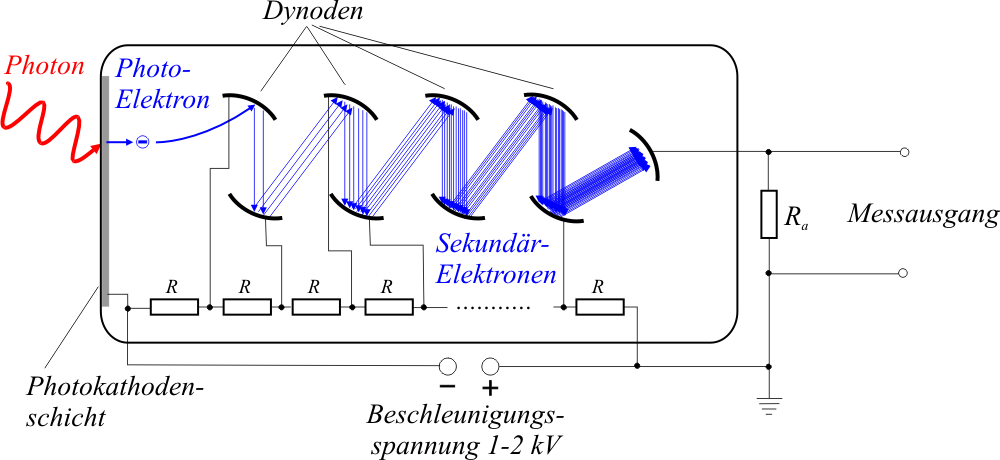
\includegraphics[width=0.85\textwidth]{images/Photomultiplier_schema_de.png}
	\caption{Schematik Photoelektronenvervielfacher}
	\label{theorie_PEV}
\end{figure}

Dort werden durch das Szintillationsphoton Elektronen aus einer Photokathode ausgeschlagen, durch angelegte Spannung zur ersten Dynode beschleunigt wo sie mit der gewonnenen kinetischen Energie weitere Elektronen auschlagen. Dieser Prozess wird einige male wiederholt bis ein messbarer elektrischer Impuls an der Anode entstehen kann.

\subsubsection{Compton-Streuung}

\subsection{Weitwinkel-Compton-Koinzidenz-Methode}

\section{Invariante Masse des $Z$-Boson}

In diesem Versuchsteil soll die invariante Masse von $Z^0 \rightarrow e^+ e^-$ Ereignissen berechnet werden.
Dies soll einmal exakt und einmal mit der Näherung $m_e = 0$ durchgeführt werden.
Für die Berechnung standen mehrere aufgenommene Detektorereignisse zur Verfügung, von denen zur Berechnung vier zufällig ausgewählt wurden.
Die invariante Masse beim Zerfall eines Teilchens in zwei Teilchen, ergibt sich mithilfe ihrer Vierervektoren zu:
\[
M^2 =\left[ \left( \begin{array}{c} E_1 \\ {\vec{p}_1} \end{array} \right) + \left( \begin{array}{c} E_2 \\ {\vec{p}_2} \end{array} \right) \right]^2
\]
\[
= m_1^2 + m_2^2 + 2 E_1 E_2 - 2 \textbf{p}_1 \textbf{p}_2 \cos \vartheta
\]
Die Energie ergibt sich aus der relativistischen Energie-Impuls-Relation zu:
\[
E_i = \sqrt{m_i^2 + \textbf{p}_i^2}
\]
Im Falle masseloser Teilchen, bzw. bei Vernachlässigung der Masse, vereinfacht sich die invariante Masse zu:
\[
M = \sqrt{2 \textbf{p}_1 \textbf{p}_2 (1-\cos \vartheta)}
\]

Hier sind $ \textbf{p}_i$ die Beträge der Impulse der Teilchen und $\vartheta$ ist der Winkel zwischen den Impulsvektoren.

Die Masse von Elektronen und Positronen beträgt: $m=511$ keV.
Zusammen mit den gegebenen Daten ergaben sich folgende invariante Massen:
\begin{center}
\begin{tabular}{ c | c| c | c | c | c }
Ereignis & $ \textbf{p}_1$ [GeV] & $ \textbf{p}_2$ [GeV] & $ \cos \vartheta $ & $M_{exakt}$ [GeV] &$ M_{m_e = 0}$ [GeV] \\ 
\hline
13 & 68,981 & 16,531 & -0,616 & 60,70137 & 60,70139 \\ 
16 & 49,689 & 60,917 & -0,140 & 83,06829 & 83,06830 \\
19 & 78,577 & 101,006 & 0,669 &72,48034 & 72,48037 \\
21 & 52,582 & 65,152 & 0,573 & 54,06895 & 54,06897 \\
\end{tabular}
\end{center}
Die Angabe der Nachkommastellen der invarianten Masse zeigt hier nicht die Messgenauigkeit, sondern soll die Unterschiede in der Berechnung zeigen.
Als Mittelwert ergibt sich eine Masse von $(67 \pm 11)$ Gev.

Wie zu sehen ist, bewirkt die Vernachlässigung der Masse in diesem Fall erst einen Unterschied in der sechsten Nachkommastelle, was für die Praxis kaum relevant ist und unter Umständen völlig von anderen Messunsicherheiten überdeckt wird.
Das ist auch nicht verwunderlich, da die Masse des Z-Bosons und damit auch die Energie die beim Zerfall zur Verfügung steht bei $91$ GeV liegt, während die Masse des Elektrons bei $511$ keV liegt.

Jetzt könnte als Frage aufkommen, warum die invarianten Massen doch recht weit von der Masse des Z-Bosons entfernt liegen.
Das Z-Boson äußert sich in der Messung als Resonanz mit endlicher Breite.
Aufgrund dieser Breite kann die Masse auch nicht exakt bestimmt werden, die gemessenen Werte werden um den wahren Wert gestreut.
Der Mittelwert von $M$ bei einer genügend großen Anzahl Messungen sollte dann jedoch der Z-Masse entsprechen.
\clearpage

\section{Mystery Datensatz}

In diesem Versuchsteil wurden mehrere Datensätze eines unbekannten Ereignisses im Atlasdetektor vorgegeben.
Aufgabe war es, anhand der sichtbaren, markanten Eigenschaften, auf das zu Grunde liegende Ereignis zu schlussfolgern. 
Die Datensätze wurden dabei jedoch so vorselektiert, dass stets mindestens zwei Leptonen ($e$ oder $\mu$) vorhanden waren.
Im Versuch wurde Datensatz 12 verwendet.
Einige Beispielhafte Detektoraufnahmen des Datensatzes sind in Abb. \ref{mysterydata} dargestellt.
Zusätzlich wurden folgende mögliche Ereignisse vorgegeben:
\begin{itemize}
\item $t \overline{t}$
\item $b \overline{b}$
\item ZZ
\item WZ
\item Z $\rightarrow \tau \overline{\tau}$
\item H $\rightarrow \tau \overline{\tau}$
\end{itemize}


Als Ereignis haben wir hier den ZZ-Zerfall identifiziert.
Zur Begründung rekapitulieren wir die möglichen Zerfallskanäle:
Das Top-Quark zerfällt in 96\% aller Fälle in ein Bottom-Quark, ein Lepton und ein Neutrino.
Danach ist der weitere Zerfallsweg, aufgrund des Bottom-Quarks, weitgehend identisch zum $b \overline{b}$ Ereignis.
Da das Bottom-Quark über die starke Wechselwirkung zerfallen kann, muss es bei diesen Ereignis häufige hadronische Schauer geben, die im hadronischen Kalorimeter deutlich zu sehen sein müssten.
Da dies offenbar nicht zu sehen ist (siehe Abb. \ref{mysterydata}), können beide Ereignisse ausgeschlossen werden.

Das Z-Boson kann, unter der Vorgabe dass zwei Leptonen entstehen, hier nur in ein Lepton-Antilepton-Paar zerfallen.
Beim ZZ-Ereignis wäre jedoch daneben noch der Zerfall in ein Neutrino-Antineutrino-Paar möglich.

Dass W-Boson hat leptonische Zerfallskanäle, in Lepton und Antineutrino sowie hadronische in ein Quark und ein Antiquark.
Da das W-Boson eine Ladung besitzt, muss beim WZ Ereignis, aufgrund der Ladungserhaltung, eine überschüssige Ladung vorhanden sein.
Dies wurde in den Datensätzen nicht beobachtet, weshalb auch diese Ereignis ausgeschlossen wurde.
Zusätzlich gegen dieses Ereignis spricht, dass das W-Boson hier einen hadronischen Zerfallsweg besitzen kann.
Da jedoch wie gesagt keine großen hadronischen Schauer zu sehen waren, spricht auch das gegen dieses Ereignis.

Zuletzt betrachten wir die Zerfälle des Z- und Higgs-Bosons in 2 Tauonen.
Tauonen zerfallen entweder in ein leichteres Lepton sowie 2 Neutrinos oder, was bevorzugt geschieht, auf hadronischen Weg.
Da hier jedoch beim Zerfall 2 Leptonen entstehen müssen, ist der hadronische Zerfall ausgeschlossen.
Damit ergeben sich hier als Zerfallsprodukte: 2 Leptonen, 2 Neutrinos und 2 Antineutrinos.
Aufgrund der entstehenden Neutrinos beim Zerfall der Tauonen, sollte hier häufig eine nennswerte fehlende transversale Energie vorhanden sein. 
Da beim ZZ Ereignis Neutrinos nicht unbedingt entstehen müssen, wäre eine Unterscheidung anhand der fehlenden Energie möglich.
Es war auch zu sehen, dass diese in den Daten ab und zu recht hoch und ab und zu quasi nicht vorhanden war, was für das ZZ Ereignis spricht.

Ein zusätzliches Argument für das ZZ Ereignis lässt sich bei Betrachtung der detektierten Myonen sehen.
Da die Zerfallswahrscheinlichkeiten in Elektronen bzw. Myonen gleich sind, würden wir beim Zerfall eines einzelnen $Z$ in $50\%$ der Fälle ein Elektron und 1 Myon erwarten und sonst jeweils 2 Elektronen oder 2 Myonen.
Beim Zerfall zweier $Z$-Bosonen würden wir demzufolge entweder 0, 2 oder 4 Myonen, aber meist (wenn kein $Z$ in ein Neutrinopaar zerfallen ist) vier Jets erwarten.
Tauonen wiederum können nicht in zwei Myonen zerfallen.
Hier würden wir also entweder 0, 1 oder 2 Myonen und stets zwei Jets erwarten.
Ein einzeln Myon wurde in den Ereignissen nicht gefunden, dafür aber einzelne Ereignisse mit vier Myonen und meist zwei oder vier Jets (siehe Abb. \ref{mytserydata}), was wieder für das ZZ Ereignis spricht.

\begin{figure}[h]
\begin{subfigure}{.8\textwidth}
\centering
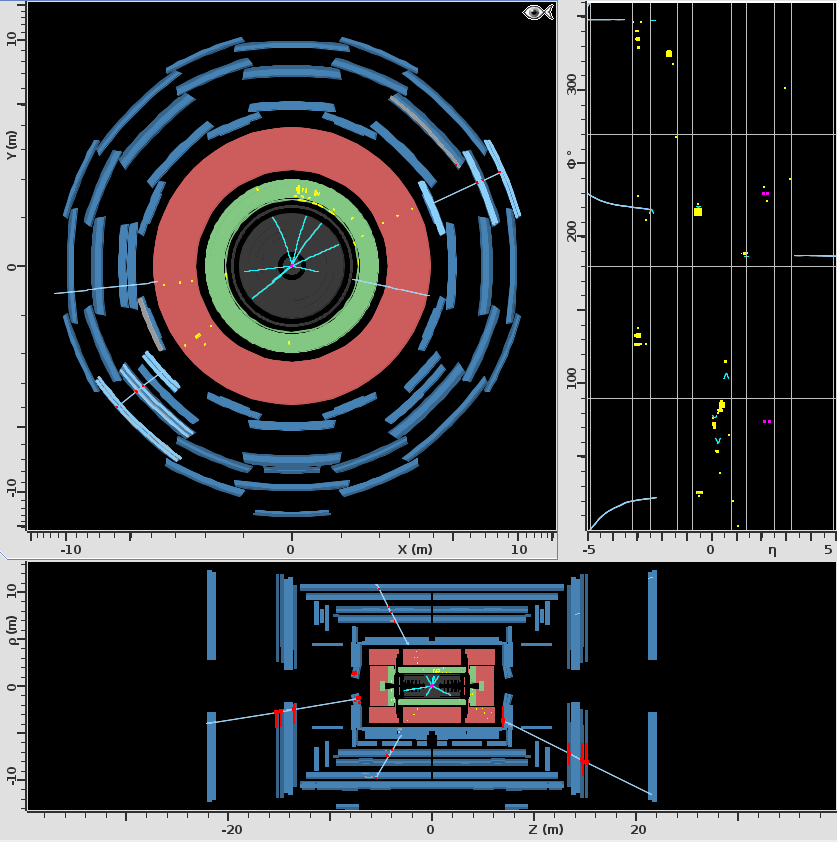
\includegraphics[width=.8\linewidth]{../Pictures/MysteryEvent2.png}
\caption{Ereignis 2}
\end{subfigure}%
\vskip\baselineskip
\begin{subfigure}{.8\textwidth}
\centering
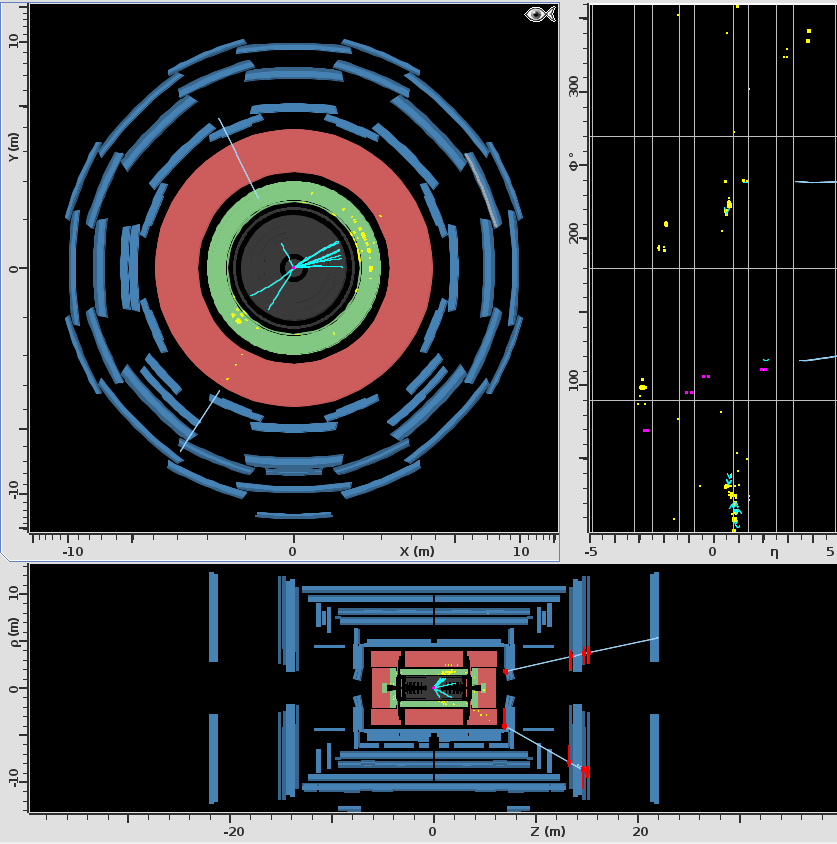
\includegraphics[width=.8\linewidth]{../Pictures/MysteryEvent16.png}
\caption{Ereignis 16}
\end{subfigure}%
\vskip\baselineskip
\begin{subfigure}{.8\textwidth}
\centering
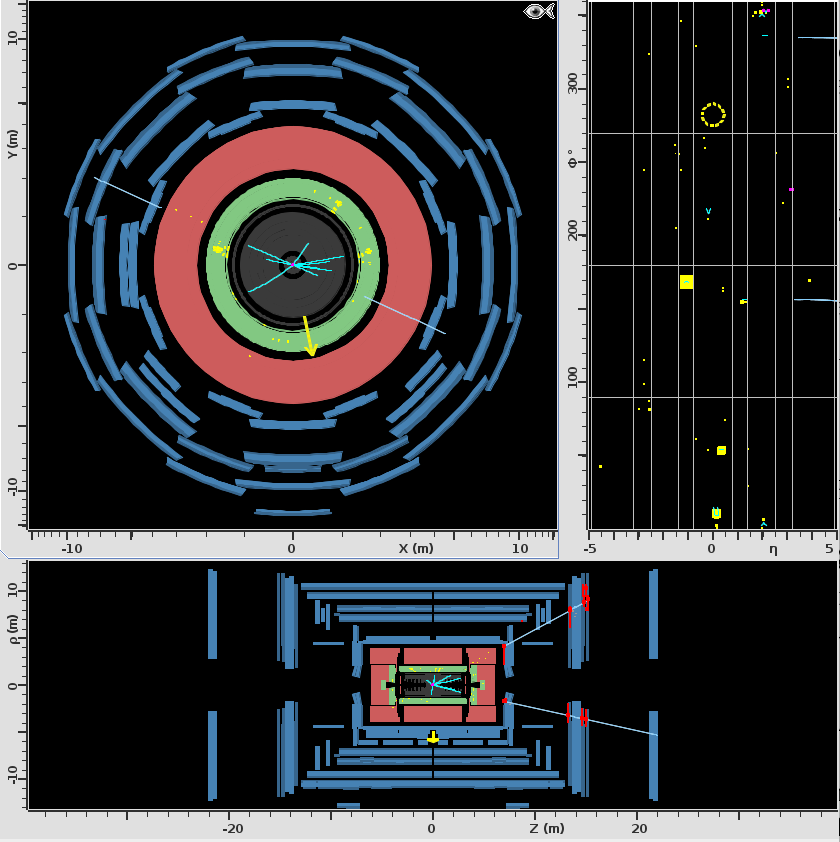
\includegraphics[width=.8\linewidth]{../Pictures/MysteryEvent21.png}
\caption{Ereignis 21}
\end{subfigure}%
\caption{Beispielhafte Ereignisse der Mysterydaten}
\label{mysterydata}
\end{figure}

\clearpage
\section{$H \rightarrow WW$ Analyse}

In diesem Versuchsteil soll die Existenz des Higgs-Bosons überprüft werden.
Dafür müssen wir zuerst vermutete Higgs-Ereignisse innerhalb unserer Daten finden.
Diese sind jedoch relativ selten, weshalb wir einen großen Untergrund haben.
Die erste Aufgabe bestand daher darin, Cuts aus physikalischen Überlegungen herzuleiten und zu implementieren, die Higgs-Ereignisse vom Untergrund trennen.

Zum Testen von Cuts stand uns die Seite \url{http://opendata.atlas.cern/visualisations/analyser-js.php} zur Verfügung.
Diese enthalt eine Mischung aus simulierten und realen ATLAS-Daten, innerhalb derer wir Cuts implementieren und deren Auswirkungen testen können.
Die dortigen Daten enthalten neben den gewünschten $H \rightarrow WW$ Ereignissen noch einen Untergrund aus $WW$, $t\overline{t}$ und $Z$ Ereignissen.
In Abb. \ref{test_nocuts} sind die Ereignisse ohne Cuts zu sehen.


\begin{figure}[h]
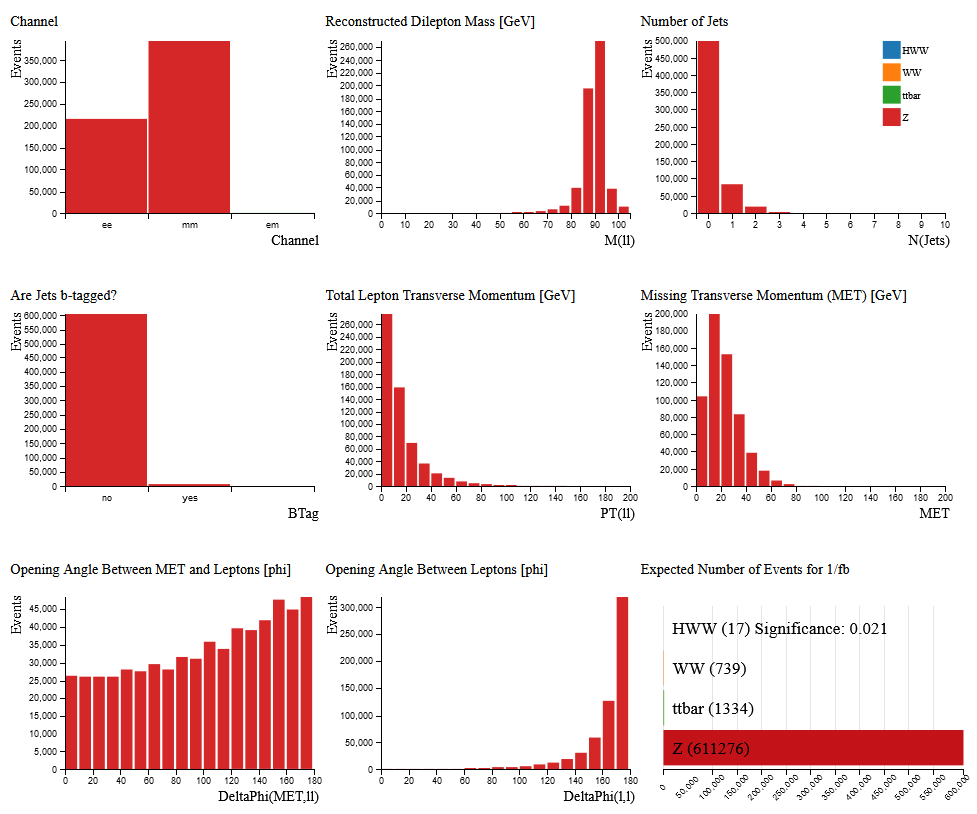
\includegraphics[width=\linewidth]{../Pictures/test_nocuts.png}
\caption{Daten ohne Cuts \cite{opendata}}
\label{test_nocuts}
\end{figure}

\clearpage

Wie zu sehen ist, werden diese Daten von einem riesigen $Z$ Untergrund dominiert.
Auf 17 $H$ Ereignisse kommen hier 611.276 $Z$ Ereignisse, was die Notwendigkeit von Cuts noch einmal verdeutlicht.
Andere Untergrundereignisse die hier betrachtet werden, sind $t\overline{t}$ (1443) und $WW$ (739) Ereignisse.
Als Maß für die Qualität unserer Cuts betrachten wir im Folgenden die Signifikanz der Higgs-Ereignisse, die ohne Cuts bei 0,021 liegt.

Für die ersten Cuts rekapitulieren wir wieder die Zerfallskanäle:
Das Z-Boson zerfällt bevorzugt in ein Lepton-Antilepton-Paar oder auf hadronischem Weg.
Dabei werden zwei gleiche Leptonen ($ee$ oder $\mu \mu$) als Endprodukt verbleiben.
Beim Zerfall zweier W-Bosonen können gemischte Endzustände ($e \mu$) existieren.
Ein Cut der nur gemischte Endzustände betrachtet, sollte also einen guten Anteil des Z-Untergrunds beseitigen (siehe Channel in Abb. \ref{test_firstcuts}).
Zusätzlich sollte der Endzustand genauso wie wie der Endzustand elektrisch Neutral sein, was innerhalb dieser Daten nicht von Relevanz ist, aber später genutzt wird.
Das Ergebnis dieses ersten Cuts ist in Abb. \ref{mixed} zu sehen.
Die ausgegrauten Ereignisse wurden hier gecutted.

\begin{figure}[h]
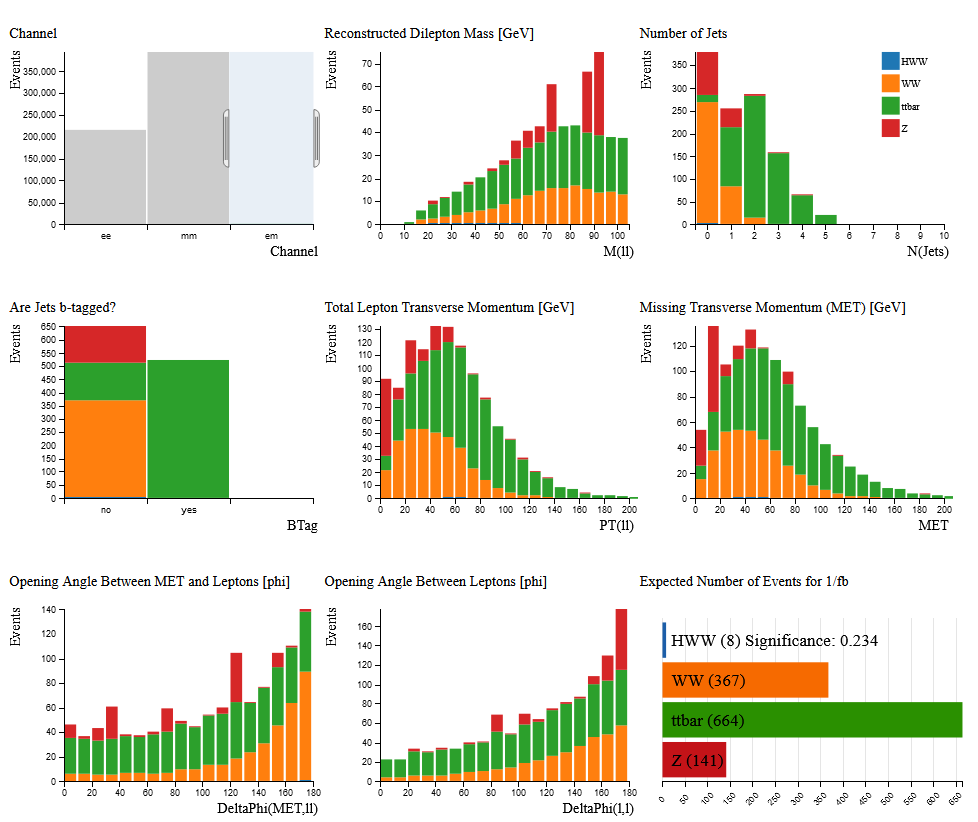
\includegraphics[width=\linewidth]{../Pictures/mixed.png}
\caption{Nur gemischte Leptonen \cite{opendata}}
\label{mixed}
\end{figure}

\clearpage

Wie wir sehen können, wurde der Z-Untergrund massiv reduziert.
Ebenfalls ein sinnvoller erster Cut würde darin bestehen, b-Jets zu ignorieren, da diese vor allem von $t\overline{t}$ Ereignissen stammen sollten.
Da wir die Masse des Higgs-Bosons ($125$ GeV) bereits kennen bietet es sich auch an Cuts an die invariante Leptonenmasse zu legen.
Hier ist jetzt jedoch zu beachten, dass bei gemischten Leptonenereignissen Neutrinos entstanden sein müssen, die nicht im Detektor gemessen werden können.
Deshalb sollte die invariante Masse niedriger als die bekannte Higgs-Masse angesetzt werden.

Ein Ergebnis dieser beschriebenen Cuts ist in Abb. \ref{test_firstcuts} zu sehen.

\begin{figure}[h]
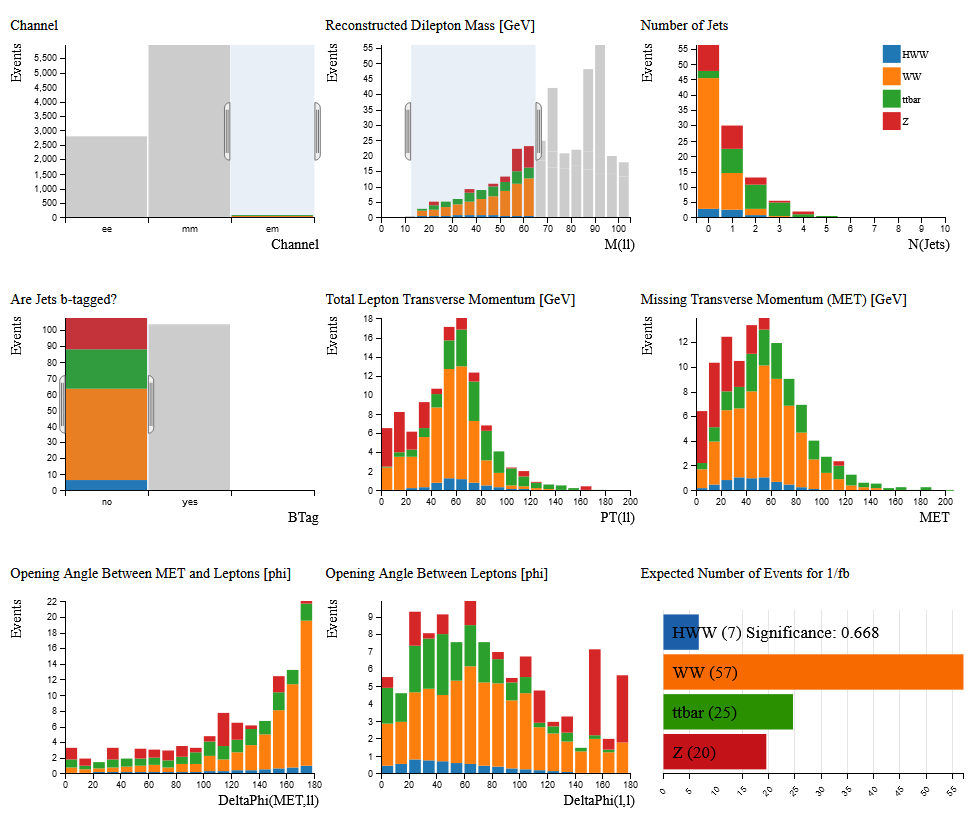
\includegraphics[width=\linewidth]{../Pictures/test_firstcuts.png}
\caption{Daten mit ersten Cuts \cite{opendata}}
\label{test_firstcuts}
\end{figure}

Als Ergebnis dieser ersten Cuts können wir sehen, dass der $Z$-Untergrund wesentlich reduziert wurde, auf nur noch 20 Ereignisse.
Gleichzeitig haben wir zwar auch 10 unserer Higgs-Ereignisse verloren, die Signifikanz hat sich jedoch aufgrund des reduzierten Untergrunds auf 0,668 erhöht.
Der Restuntergrund wird vor allem von 57 $WW$-Ereignissen dominiert.
Diese sollten von Natur aus recht schwer von $H \rightarrow WW$ Ereignisse zu trennen sein.
Weitere Cuts die angesetzt wurden, zielten darauf aus höhere fehlende transversale Energien, höhere Jet-zahlen oder niedrige Winkel zwischen den Leptonen zu reduzieren.
Dies alles hatte jedoch nur noch kleinere Auswirkungen, mit weiteren Cuts war nur noch eine Steigerung der Signifikanz auf 0,743 möglich (siehe Abb. \ref{test_secondcuts}.
Mit Blick auf die Daten ist eine weitere Erhöhung der Signifikanz scheinbar nicht möglich.

Zusammenfassend haben wir also von Ursprünglich über 600.000 Ereignissen, unter denen sich 17 Higgs-Ereignisse mit einer Signifikanz von 0,021 befanden, nach Implementierung der Cuts noch 37 mit 4 Higgs-Ereignissen, die jetzt jedoch eine Signifikanz von 0,743 besitzen.
Der verbliebende Untergrund besteht 24 $WW$, 9 $t\overline{t}$.
Der $Z$-Untergrund konnte vollständig beseitigt werden.
Eine vollständige Beseitigung des $WW$ Untergrundes erscheint ohne weitere Berechnungen nicht realistisch, aufgrund der Ähnlichkeit zum $H \rightarrow WW$.
Möglicherweise wäre jedoch noch mit besseren Cuts eine komplette Beseitigung der $t\overline{t}$ Ereignisse möglich.

\begin{figure}[h]
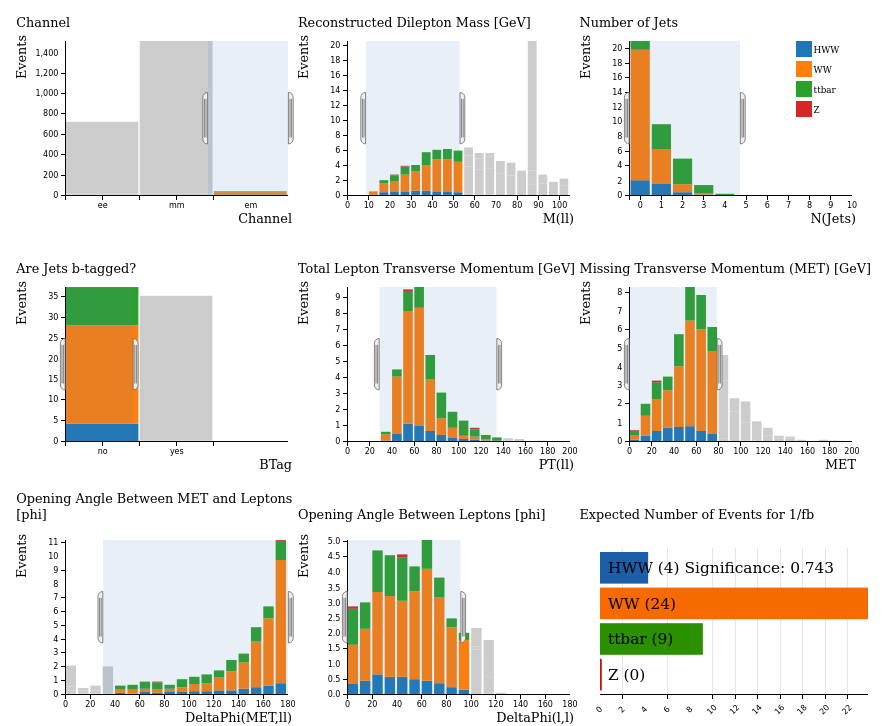
\includegraphics[width=\linewidth]{../Pictures/test_secondcuts.png}
\caption{Finale Cuts \cite{opendata}}
\label{test_secondcuts}
\end{figure}

\clearpage

Die so getesteten Cuts wurden im Folgenden auf die uns zur Verfügung stehenden Daten angewandt.
Als Maß nutzen wir nun keine Signifikanz, sondern das Verhältnis von Signal zum Untergrund (S/B in den Abbildungen) sowie von Daten und Simulation (Data/MC in den Abbildungen).
In Abb. \ref{Cuts_mass} und \ref{Cuts_momentum} werden die Auswirkungen dieser Cuts schrittweise dargestellt.
Zur Anschaulichkeit beschränken wir uns in der Darstellung auf die invariante Masse und den Impuls der Leptonen, die anderen Größen wurden jedoch außerhalb des Protokolls auch im Auge behalten.
Auch hier scheinen unsere Cuts den Untergrund effektiv zu reduzieren.
Das Verhältnis zwischen Daten und Simulation konnte ebenfalls in dem Bereich in dem Higgs-Bosonen auftreten auf Werte nahe 1 gebracht werden, wobei dieses außerhalb der Bereiche schnell deutlich schlechtere Werte annimmt.
Zu beobachten ist ebenfalls, dass der Fehler innerhalb der Daten sich mit Anzahl der Cuts erhöht, was jedoch zu erwarten ist.

\begin{figure}[h]
\begin{subfigure}{.5\textwidth}
\centering
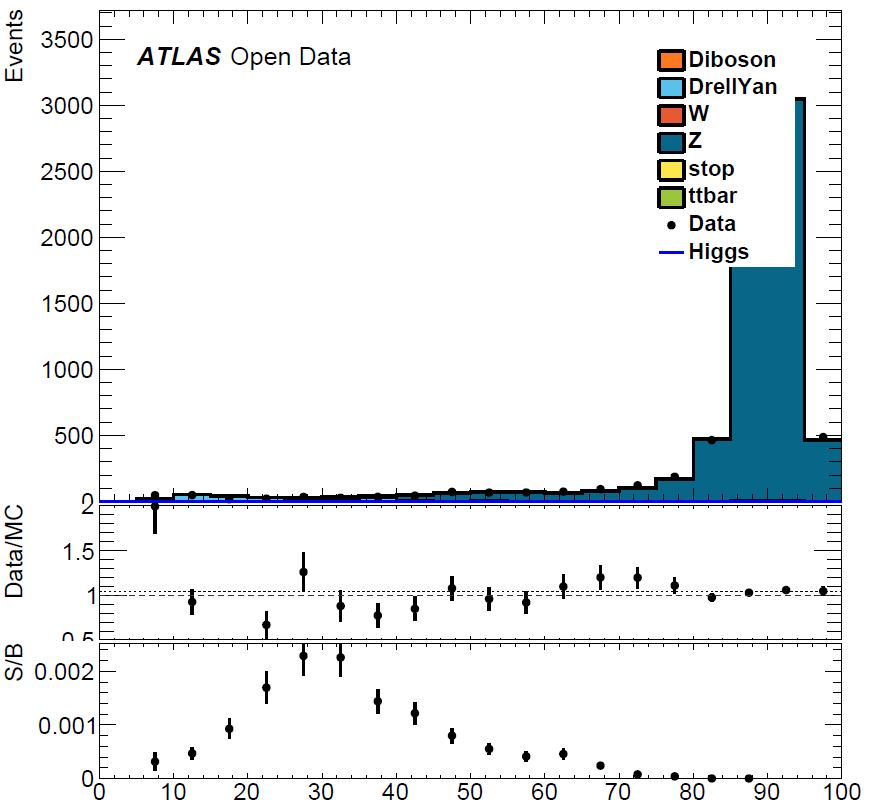
\includegraphics[width=.8\linewidth]{../Pictures/nocuts_mass.png}
\caption{Daten ohne Cuts}
\end{subfigure}%
\begin{subfigure}{.5\textwidth}
\centering
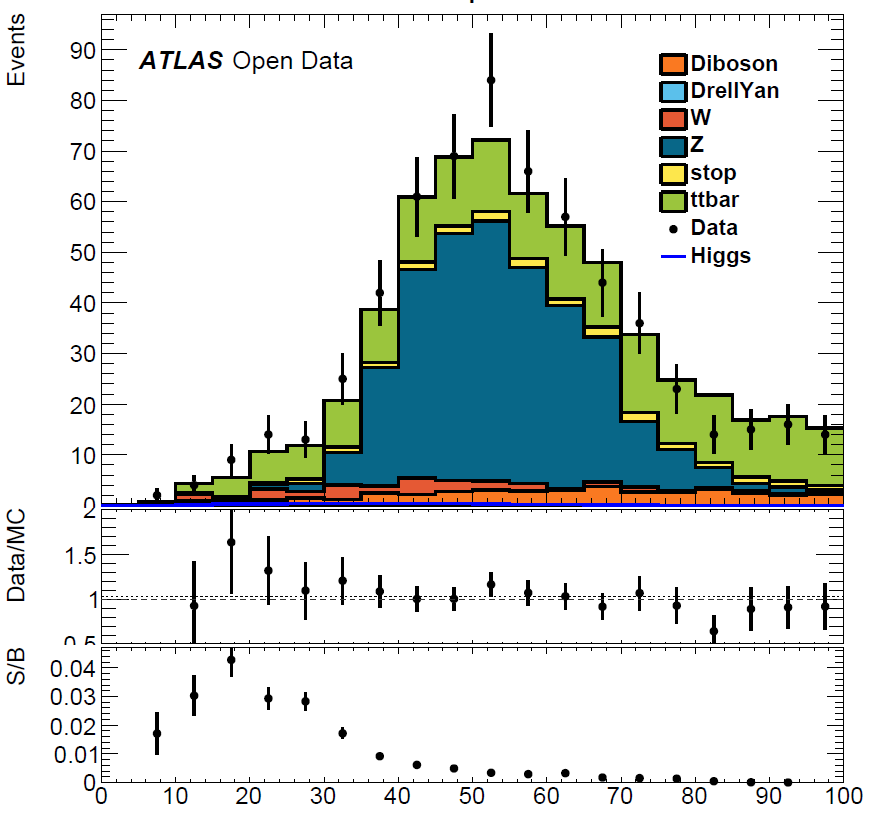
\includegraphics[width=.8\linewidth]{../Pictures/1cut_mass.png}
\caption{Nur gemischte Leptonen und kein Ladungsüberschuss}
\end{subfigure}%
\vskip\baselineskip
\begin{subfigure}{.5\textwidth}
\centering
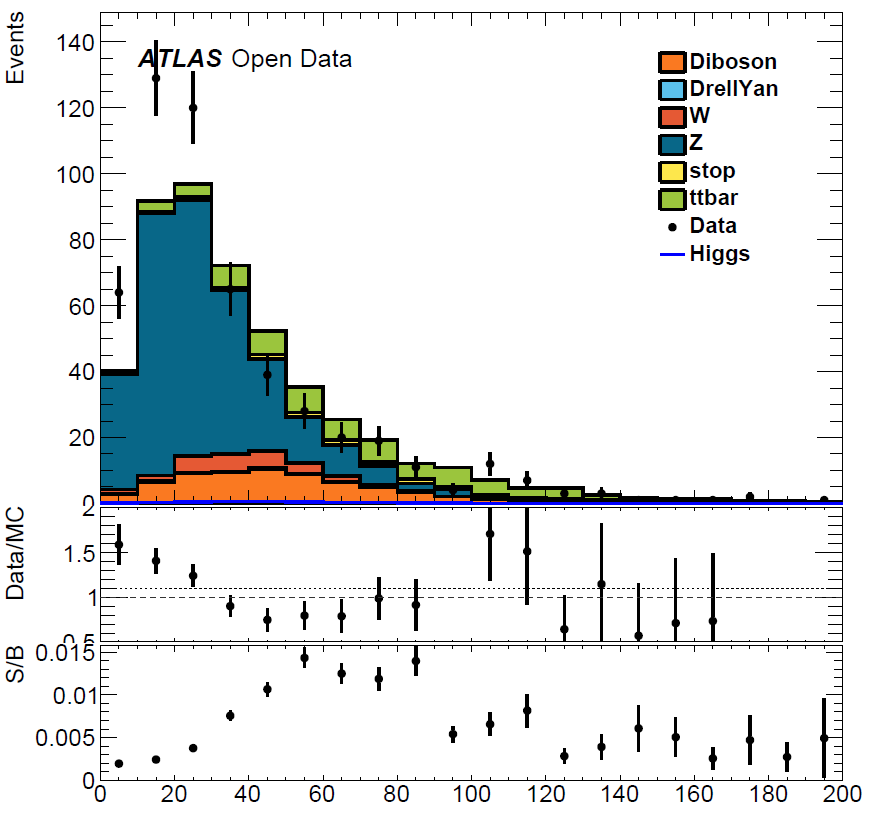
\includegraphics[width=.8\linewidth]{../Pictures/2cut_mass.png}
\caption{Cut aller b-Jets}
\end{subfigure}%
\begin{subfigure}{.5\textwidth}
\centering
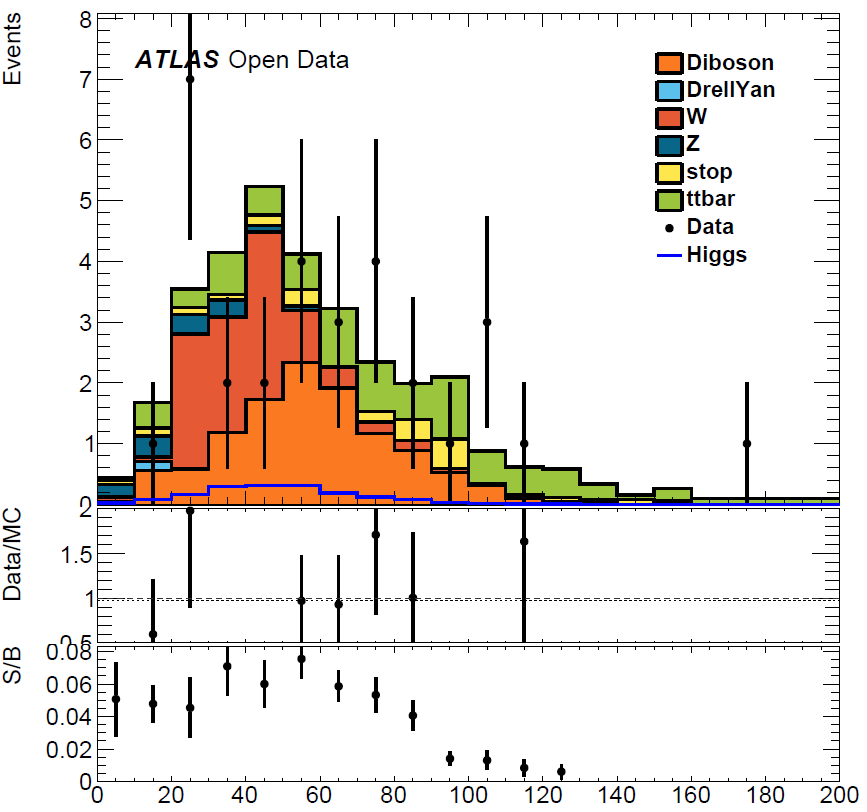
\includegraphics[width=.8\linewidth]{../Pictures/3cut_mass.png}
\caption{weitere Cuts}
\end{subfigure}%
\caption{Auswirkungen der Cuts auf die Ereignisse unter Betrachtung der invarianten Masse}
\label{Cuts_mass}
\end{figure}

\begin{figure}[h]
\begin{subfigure}{.5\textwidth}
\centering
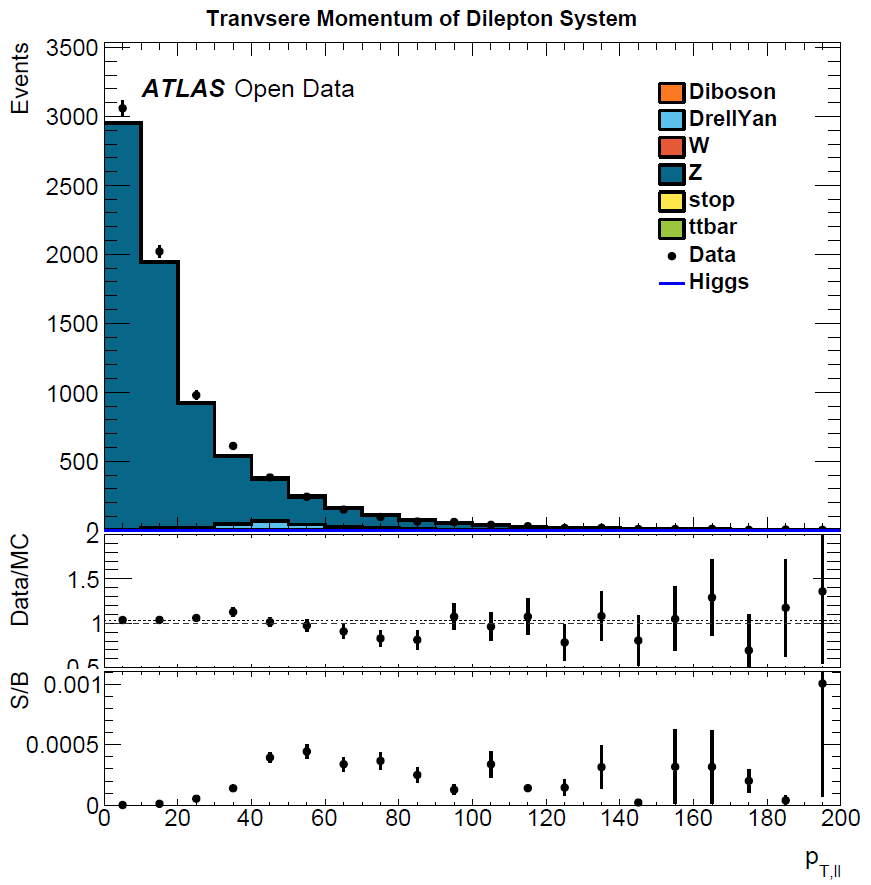
\includegraphics[width=.8\linewidth]{../Pictures/nocuts_momentum.png}
\caption{Daten ohne Cuts}
\end{subfigure}%
\begin{subfigure}{.5\textwidth}
\centering
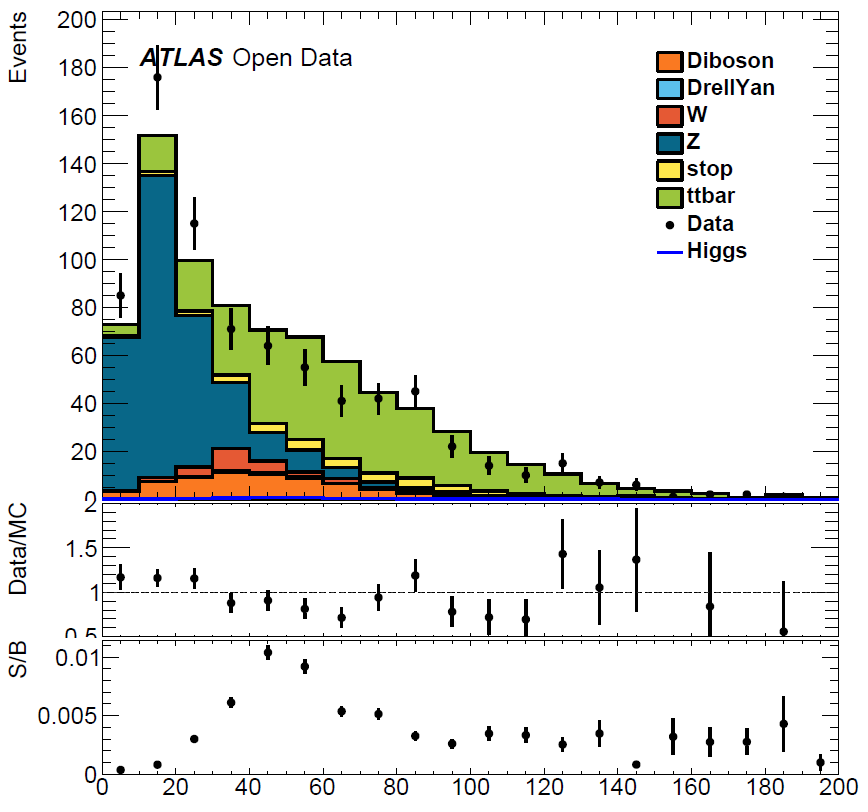
\includegraphics[width=.8\linewidth]{../Pictures/1cut_momentum.png}
\caption{Nur gemischte Leptonen und kein Ladungsüberschuss}
\end{subfigure}%
\vskip\baselineskip
\begin{subfigure}{.5\textwidth}
\centering
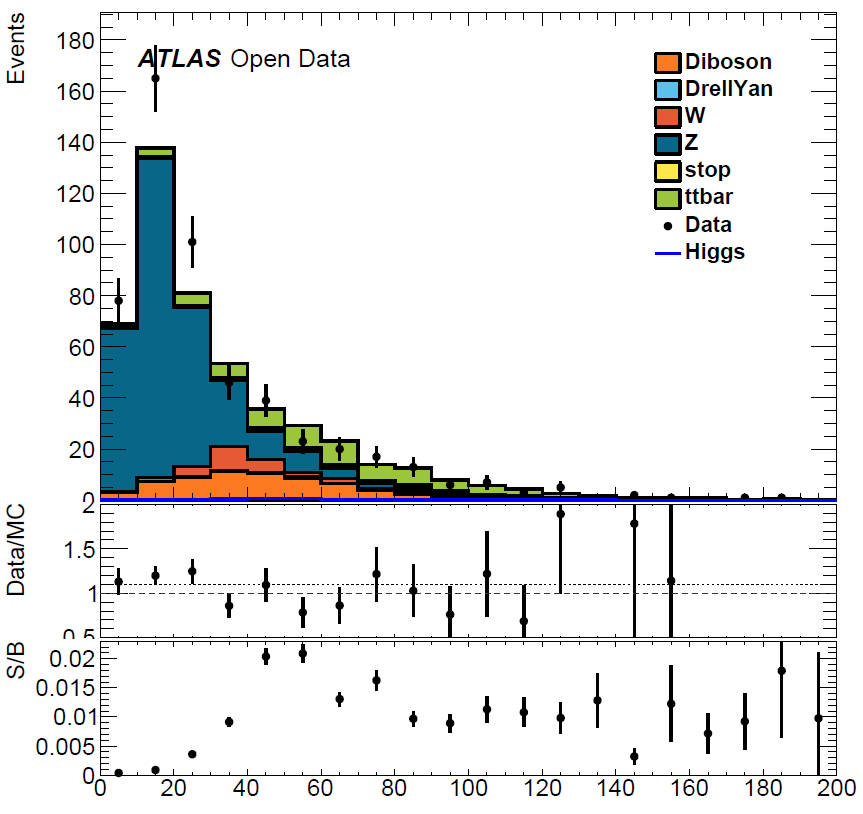
\includegraphics[width=.8\linewidth]{../Pictures/2cut_momentum.png}
\caption{Cut aller b-Jets}
\end{subfigure}%
\begin{subfigure}{.5\textwidth}
\centering
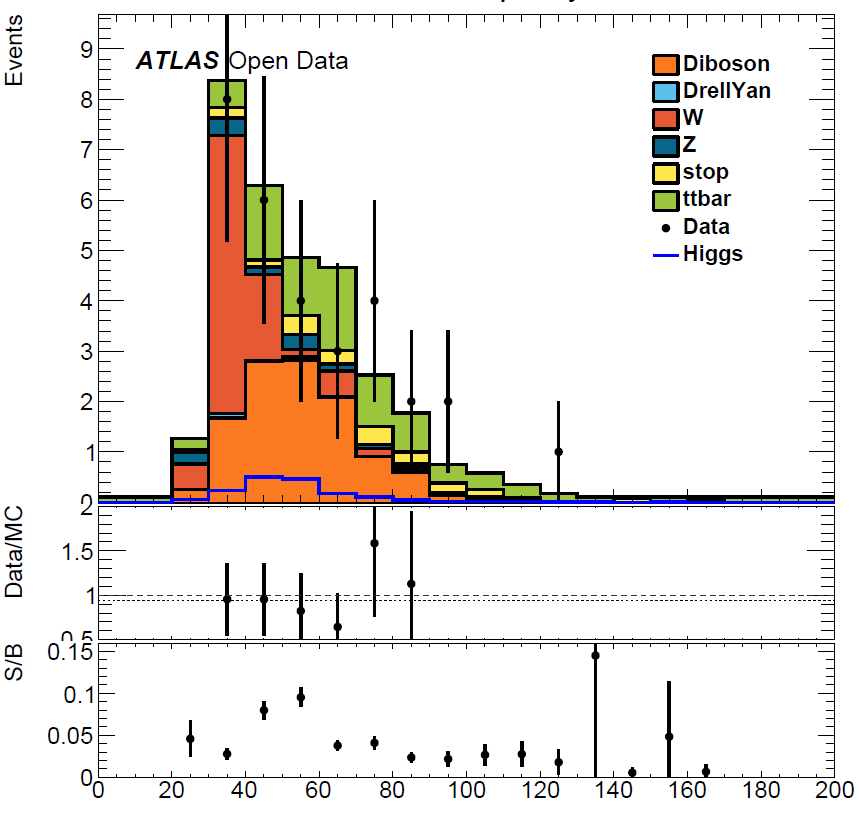
\includegraphics[width=.8\linewidth]{../Pictures/3cut_momentum.png}
\caption{weitere Cuts}
\end{subfigure}%
\caption{Auswirkungen der Cuts auf die Ereignisse unter Betrachtung des Leptonenimpulses}
\label{Cuts_momentum}
\end{figure}

Ausgehend von diesen Daten wurde nun zur statistischen Analyse der p-Value berechnet.
Für diese Berechnung wurden 10000 Pseudoexperimente durchgeführt.
Als Ergebnis ergaben sich ein p-Value von 0.0039 und eine obere Grenze für $\mu$ von 1.
Nach Konventionen der Teilchenphysik, ist ein p-Value von $5,7 \cdot 10^{-7}$ (entspricht $5 \sigma$) notwendig um von der Entdeckung eine Teilchens zu sprechen, dies ist hier offenbar nicht der Fall.
Ein p-Value von $0,05$ ($2 \sigma$) ist jedoch bereits ausreichend um die Nullhypothese, also die Nichtexistenz des Higgs-Bosons, zu verwerfen.
Dies ist hier offenbar der Fall, sodass wir davon ausgehen können, dass unsere Daten in guter Übereinstimmung mit dem Standardmodell mit Higgs-Boson sind.
\section{Suche nach neuer Physik}

In diesem letzten Versuchsteil soll nun innerhalb unserer Daten nach neuer Physik, genauer gesagt nach dem $Z'$-Boson gesucht werden.
Genauer wird nach einem $Z'$ gesucht, das in ein $t \overline{t}$ Paar zerfällt.
Dafür stehen wieder Monte-Carlo-Simulationen zur Verfügung, die solche Zerfälle für verschiedene Massen des $Z'$ im Bereich von 400 bis 3000 GeV simulieren.
Wie bei der Higgs-Analyse sollen dafür als erstes wieder Cuts implementiert werden.
Da dies völlig analog zur vorherigen Aufgabe geschah, werden wir auf Details dazu nicht groß eingehen und uns in dieser Auswertung vor allem auf die Ergebnisse der Cuts konzentrieren.
Im Abb.\ref{Cuts_z} sind beispielhaft die Impulse der Leptonen mit und ohne Cuts, sowie die invariante Masse dargestellt.
Hier ist zu beachten, dass die $Z'$-Ereignisse aufgrund ihrer geringen Häufigkeit um den Faktor 10 hervorgehoben wurden.
Wir können hier wieder Bereiche mit $Z'$-Ereignissen sehen.
Der Untergrund hier wird von $t \overline{t}$ Ereignissen dominiert.
Durch Auswahl unserer Cuts konnten der Untergrund wieder deutlich reduziert und die $Z'$ Ereignisse hervorgehoben werden.
Da wir für die Suche nach einem $Z' \rightarrow t \overline {t}$ Zerfall suchen, ist eine vollständige Beseitigung des $t$-Untergrundes nicht zu erwarten.
Im Bereich in dem die meisten $Z'$-Ereignisse zu erwarten sind, liegt das Verhältnis aus Daten und Untergrund wieder nahe 1, was für unsere Cuts spricht (siehe Abb. \ref{Cuts_z}.
Insbesondere bei der invarianten Masse sind die relativen Fehler hier jedoch recht hoch.
\begin{figure}[h]
\begin{subfigure}{.5\textwidth}
\centering
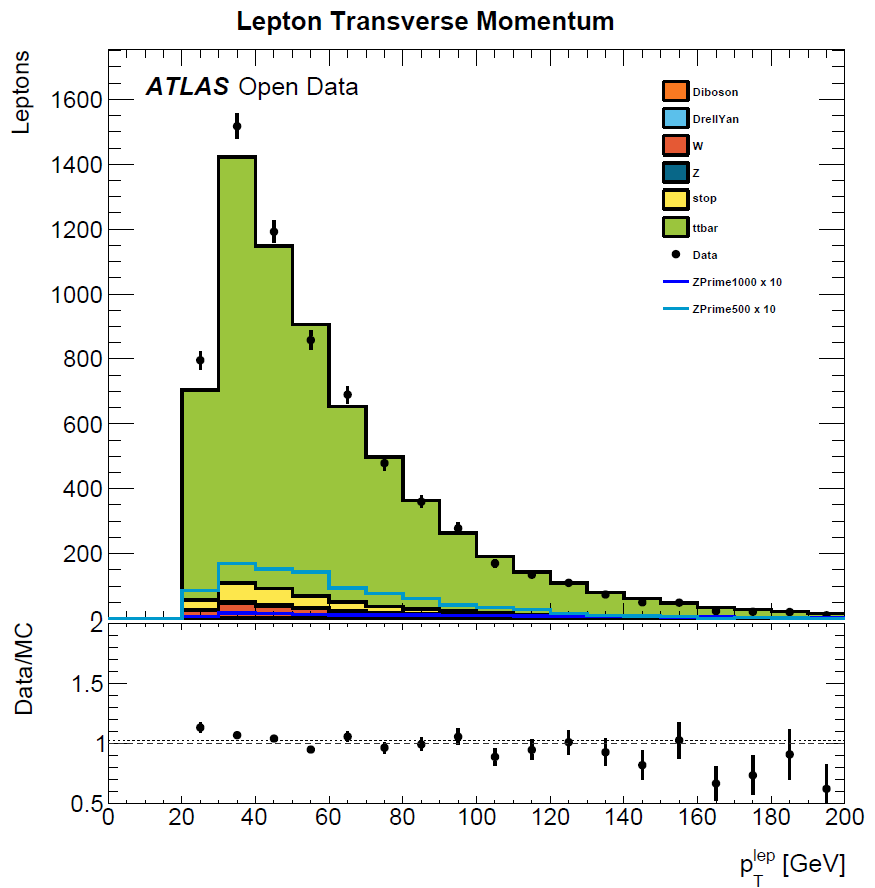
\includegraphics[width=.8\linewidth]{../Pictures/before.png}
\caption{Impulse ohne Cuts}
\end{subfigure}%
\begin{subfigure}{.5\textwidth}
\centering
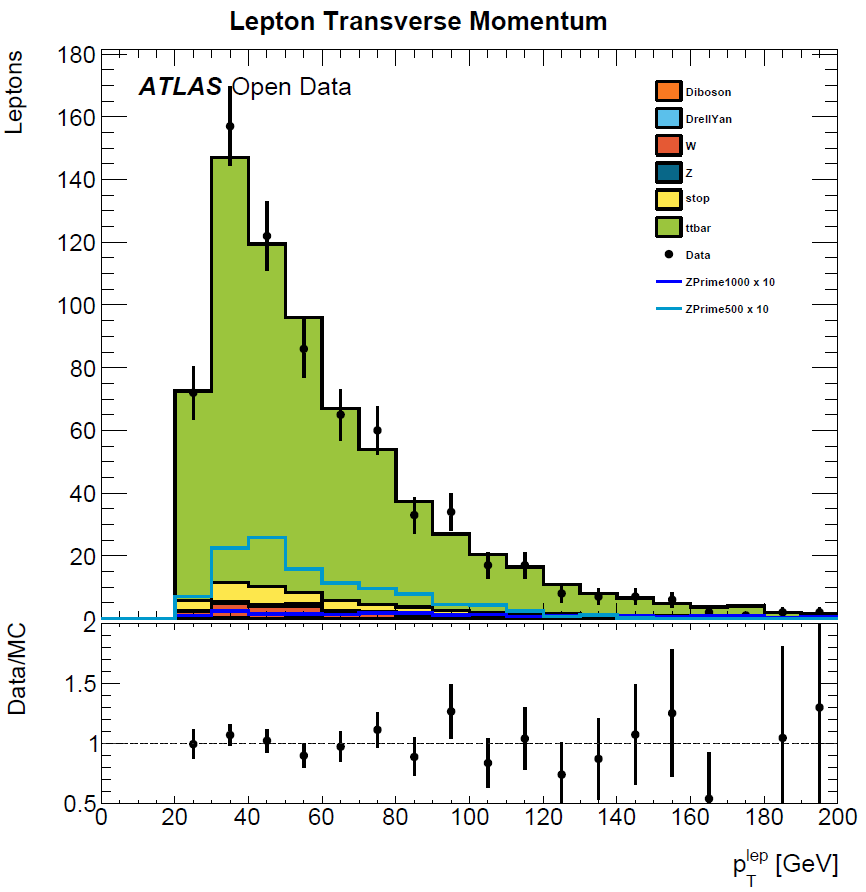
\includegraphics[width=.8\linewidth]{../Pictures/after.png}
\caption{Impulse mit Cuts}
\end{subfigure}%
\vskip\baselineskip
\begin{subfigure}{.5\textwidth}
\centering
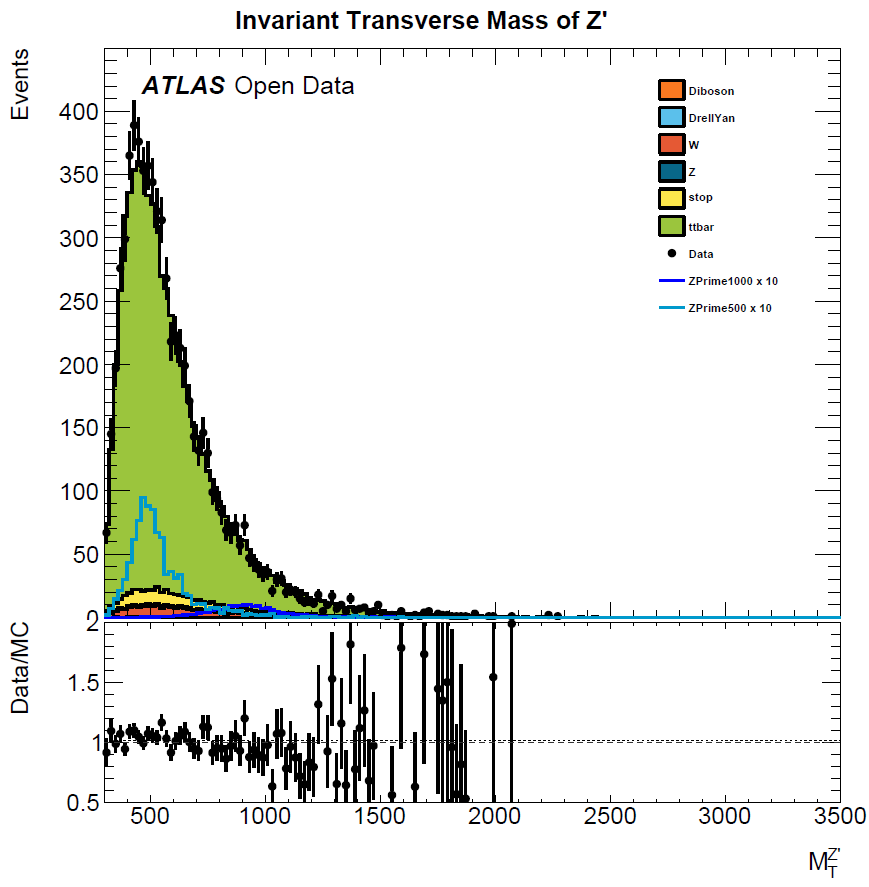
\includegraphics[width=.8\linewidth]{../Pictures/mass_before.png}
\caption{invariante Masse ohne Cuts}
\end{subfigure}%
\begin{subfigure}{.5\textwidth}
\centering
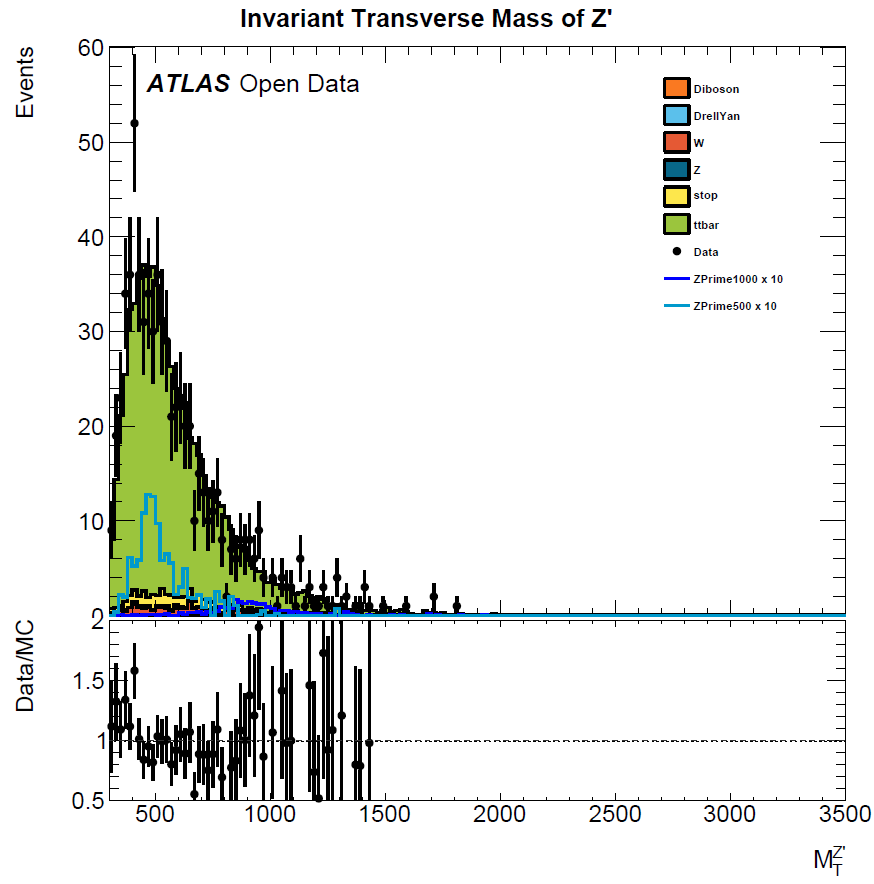
\includegraphics[width=.8\linewidth]{../Pictures/mass_after.png}
\caption{invariante Masse mit Cuts}
\end{subfigure}%
\caption{Auswirkungen der Cuts auf die Ereignisse }
\label{Cuts_z}
\end{figure}

Mit den so erhaltenen Daten wurden wieder p-Value Berechnungen für beide ausgewählte Massen durchgeführt.
Diesmal wurden für die Berechnungen jedoch nicht für das gesamte vorhandene Spektrum, sondern nur für den Bereich mit dem besten Verhältnis aus Signal und Untergrund genutzt.
Als Ergebnis ergaben sich folgende Werte:
\begin{center}
\begin{tabular}{c | c | c }
Masse [GeV] & p-Value & obere Grenze für $\mu$ \\
\hline
$400$ & 0,032 & 4,6 \\
$500$ & 0,11 & 5,2 \\
\end{tabular}
\end{center}
Alle anderen betrachteten Massehypothesen (bis zu $2500$ GeV) resultierten in p-Value Werten von $0,99...$ oder gar $1$, was sich so interpretieren lässt, dass die Daten perfekt ohne ein $Z'$ dieser Masse erklärt werden können.

Für die Interpretation erinnern wir uns an die Bedeutung des p-Values: Um von der Entdeckung eines neuen Teilchens zu reden, ist ein p-Value von $5,7 \cdot 10^{-7}$ notwendig.
Da unsere Werte deutlich höher sind, wurde also kein $Z'$-gefunden.
Ein Unterschreiten des p-Values von $0,05$ ($2 \sigma$) ist jedoch ausreichend um die Nullhypothese zu verwerfen.
Dies liegt offenbar für ein $Z'$ der Masse $400$ GeV vor.
Für die Masse von $500$ GeV wurde ein Wert von nur $0,11$ bestimmt, was für sich alleine gesehen mit hoher Wahrscheinlichkeit Rauschen entspricht.
In Kombination mit den deutlich besseren Wert für $400$ GeV kann dies jedoch als Indiz für ein Ereignis in diesem Massenbereich gesehen werden.
Dies wäre ausreichend um eine nähere Beschäftigung mit dem $Z'$ oder den Daten zu motivieren.

\clearpage
\section{Diskussion}

Alle Aufgabenteile konnten erfolgreich abgeschlossen werden.

Im Niedrigenergiebereich wurden fünf verschiedene Proben auf ihre Zusammensetzung untersucht.
Dabei konnten in der 153BeO die Teilchen $^{16}$O$^{1-}$, $^{9}$Be$^{16}$O$^{1-}$ und $^{12}$C$^{16}$O$^{1-}$ bzw. $^{28}$Si$^{1-}$ nachgewiesen werden.
In den anderen Proben konnten diverse andere Teilchen, darunter bereits erwähnte mit anderen Nukliden sowie AlO gefunden werden.
Zusätzlich wurden einige unbekannte Stoffe gefunden, die wir in diesem Praktikum nicht genauer identifizieren konnten.
Mit einer genauerem Untersuchung der Probe bzw. genaueren Wissen über potentiell vorkommende Elemente sollte das aber auch möglich sein.

Im Hochenergiebereich wurde nur eine Probe untersucht.
Bei dieser wurden die Nuklide $^{9}$Be, $^{10}$Be, $^{12}$C, $^{16}$O und $^{26}$Al in verschiedenen Ladungszuständen gefunden.
Hier ist teilweise eine recht große Ungenauigkeit zwischen berechneter Masse und dem Nuklid vorhanden.
Dies lässt sich zumindest teilweise auf die unbekannten Ungenauigkeiten der Messung zurückführen.
Möglicherweise wurden hier auch einzelne Ionen fehlgedeutet.
Mit Kenntnis der Ursache der Ungenauigkeiten könnte dies genauer werden.

Weiterhin wurde die Detektion und Identifikation von $^{10}\text{Be}$ in einer Gasgefüllten Ionisationsdetektor vorgenommen.
Eine Trennung von den meisten unerwünschten Nukliden die nach dem Beschleuniger auftreten erfolgt durch einen Ablenkmagneten und einen ESA.
Aber auch das Isotop $^{9}\text{Be}$ kann gefunden werden, obwohl man es eigentlich durch Vorselektion aussortieren wollte.
Als Ursache dafür wurde die Molekülbildung von $^{9}\text{Be}^{1}\text{H}^{2+}$ angeführt.
Die Identifikation ist trotz des Auftretens des Isobars $^{10}\text{B}$ möglich.
Es ist sogar möglich das Isobar quantitativ im Spektrum von $^{10}\text{Be}$ zu trennen, womit grundsätzlich eine genaue Bestimmung des Anteils des radioaktiven Isotops $^{10}\text{Be}$ möglich ist, und damit die eigentliche Altersbestimmung.

Die Anteilsbestimmung wurde im letzten Versuchsteil vorgenommen.
Die Konzentration des Radionuklides $^{10}$Be wurde dazu in vier verschiedenen Proben berechnet.
Die Ergebnisse dafür sind in Tab. \ref{dis_con} zu sehen.
\begin{table}[h]
\centering
\caption{Gemessene Werte zur Berechnung der $^{10}$Be Konzentration in den Proben.}
\begin{tabular}{|c |c| c|}
\hline
Probe& $\frac{\text{Atome}}{\si{\gram}}$ & mittlere Tiefe [cm] \\
\hline
KY13 &  $(\num{1.115} \pm \num{0.050}) \cdot 10^{6} $ & 47,5\\
KY14 &  $(\num{9.61} \pm \num{0.44}) \cdot 10^{5} $ & 57,5 \\
KY16 &  $(\num{7.66} \pm \num{0.36}) \cdot 10^{5} $ & 92,5\\
KY17 &  $(\num{6.23} \pm \num{0.33}) \cdot 10^{5} $ & 112,5\\
\hline
\end{tabular}
\label{dis_con}
\end{table}
Wir konnten feststellen, dass die Konzentration scheinbar linear mit zunehmender Tiefe abnimmt.
Dies haben wir so erklärt, dass $^{10}$Be durch Ereignisse mit kosmischer Strahlung entsteht und tieferliegende Proben aufgrund ihres Alters daher weniger $^{10}$Be enthalten müssen.
Nach dieser Erklärung sollte eigentlich ein exponentieller Abfall stattfinden, was wir aber weder ausschließen noch bestätigen können.
Weitere Proben zur Messung könnten diese Frage aber beantworten.
Eine Verfälschung der Proben durch hochenergetische Strahlung aus anderen Quellen ist potentiell möglich, würde aber nichts am Abnehmen der Konzentration ändern.
Eine Neutronenquelle im Inneren der Probe würde das Ergebnis entsprechend ändern können, ist aber unwahrscheinlich.


\nocite{*} % alle resourcen auflisten
\printbibliography

% ----- DOKUMENT ENDE -----

\end{document}
